\documentclass[UTF8,a4paper,10pt]{ctexart}
\usepackage{geometry,booktabs,float,graphicx,amsmath}\geometry{margin=1.9cm}\setlength{\parskip}{.2em}
\title{APMCM B题问题4--5：偏好及扰动鲁棒性（最终修订）}\author{}\date{}\begin{document}\maketitle
\section*{问题4：权重变化与偏好鲁棒设计}
固定问题3的理想点与Nadir点，定义
\[z_k(x)=\frac{F_k(x)-F_k^I}{F_k^N-F_k^I},\quad
G(x;w)=\max_k\{3w_kz_k(x)\}+10^{-4}\sum_k3w_kz_k(x),\quad
w_k\ge0,\ \sum_kw_k=1.\]
对每组权重令$G^*(w)=\min_{x\in\mathcal P_{ref}}G(x;w)$，偏好机会损失为$r_{pref}(x,w)=G(x;w)-G^*(w)$，最终模型为
\[x_{pref}^{rob}=\arg\min_{x\in\mathcal P_{ref}}\max_{w\in\mathcal W_H}r_{pref}(x,w).\]
由于$G$对三个最小化目标单调不减，被支配方案不可能优于支配它的方案，故可在问题3全局Pareto参考集上搜索。等权$w=(1/3,1/3,1/3)$下$(a,b,N)=(.224932,4.500000,6)$且$G=.386383$，与问题3严格闭合。$H=25,50,100$均给出同一最小最大遗憾方案；$\max r_{pref}=1.15896>1$并非概率异常：极端权重下$\lambda_k=3w_k$可达3，评分损失不受$[0,1]$限制。
\begin{table}[H]\centering\scriptsize\caption{精确代表权重下的专属最优解（各行评分不能横向比较）}\begin{tabular}{lrrrrrrr}\toprule 场景&a&b&N&R&P&U&G\\\midrule
均衡 & 0.2249 & 4.5000 & 6 & 0.734330 & 0.097996 & 0.790195 & 0.38638 \\
散热优先 & 0.2173 & 3.3746 & 8 & 0.729817 & 0.135464 & 0.806106 & 0.43223 \\
能耗优先 & 0.2276 & 4.5000 & 4 & 0.741093 & 0.085541 & 0.771816 & 0.31344 \\
均匀性优先 & 0.2172 & 3.4315 & 4 & 0.736923 & 0.110526 & 0.773226 & 0.25082 \\
热可靠性优先 & 0.2414 & 3.0411 & 4 & 0.730921 & 0.131229 & 0.784544 & 0.36148 \\\\\bottomrule\end{tabular}\end{table}
\begin{table}[H]\centering\scriptsize\caption{偏好遗憾与网格收敛}\begin{tabular}{lrrr}\toprule 方案&最大遗憾&平均遗憾&P95遗憾\\\midrule
问题3名义 & 1.15896 & 0.33274 & 0.83562 \\
问题4偏好鲁棒 & 1.15896 & 0.33274 & 0.83562 \\
最佳原始样本 & 1.29640 & 0.37959 & 0.95182 \\
散热优先方案 & 2.16070 & 0.82107 & 1.73720 \\
能耗优先方案 & 1.56709 & 0.24988 & 0.90412 \\
无针肋最佳 & 4.19373 & 1.67466 & 3.25123 \\\\\bottomrule\end{tabular}\quad\begin{tabular}{rrrrrr}\toprule H&权重数&a&b&N&最大遗憾\\\midrule
25 & 351 & 0.2249 & 4.5000 & 6 & 1.15896 \\
50 & 1326 & 0.2249 & 4.5000 & 6 & 1.15896 \\
100 & 5151 & 0.2249 & 4.5000 & 6 & 1.15896 \\\\\bottomrule\end{tabular}\end{table}
无针肋在1326个$H=50$权重下从未成为最优；$N=2,4,6,8,10$的区域占比分别为3.8\%、55.8\%、22.7\%、2.6\%、15.0\%。$N=4$覆盖权重区域最多，而$N=6$最小化最坏机会损失；前者衡量场景出现区域，后者衡量跨场景最坏损失，二者标准不同并不矛盾。\begin{figure}[H]\centering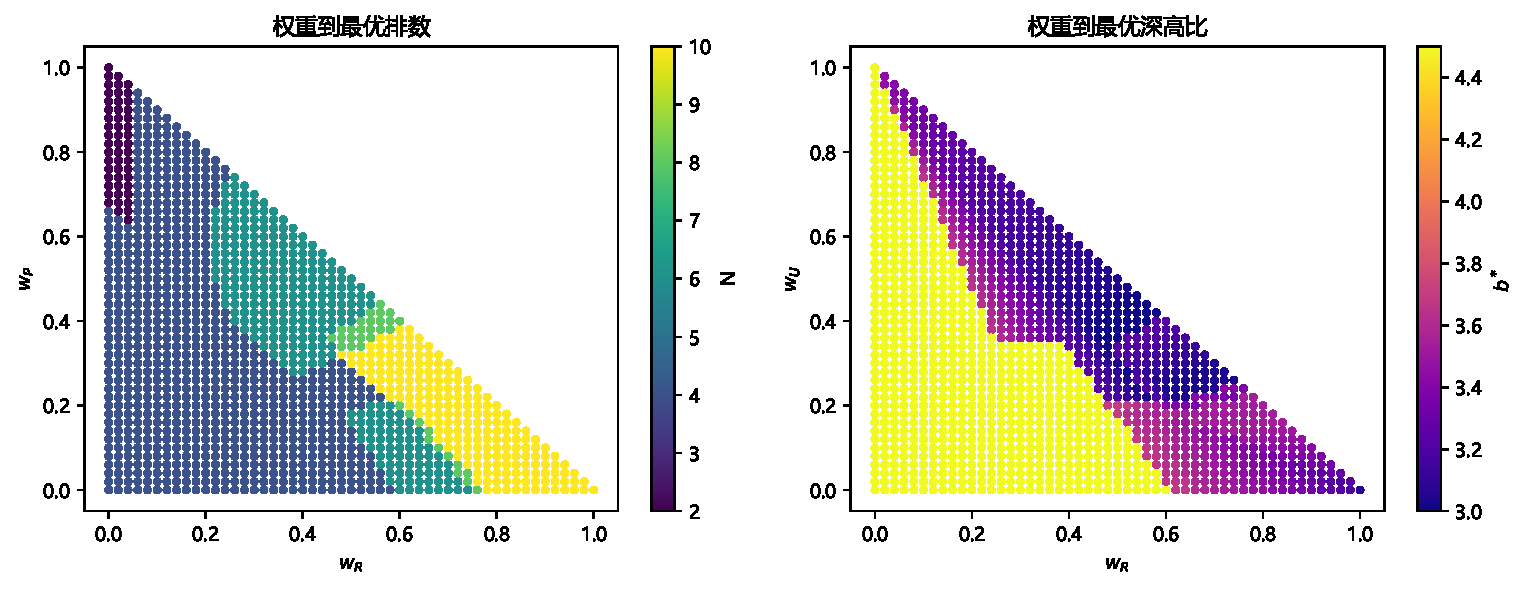
\includegraphics[width=.86\linewidth]{../../05_figures/q4/fig_q4_01_weight_mapping.pdf}\caption{权重到最优设计的映射；右图颜色表示$b^*$}\end{figure}
\section*{问题5：加工误差与工况波动}
题目未给出真实制造公差和工况波动统计，以下均为参数化中等扰动情景，只用于方案相对比较，不解释为设备实际失效概率或真实公差标准。$\varepsilon_a,\varepsilon_b\in[-.025,.025]$分别对应$|\Delta a|\le.005$和$|\Delta b|\le.0375$。
\subsection*{A类：代理模型域内的加工鲁棒结论}
中等公差为独立均匀$\varepsilon_a,\varepsilon_b\sim U[-.025,.025]$，实际尺寸$a^r=a+.20\varepsilon_a,b^r=b+1.50\varepsilon_b$。正式CVaR使用种子20260720的$L=20000$个LHS样本，40,000样本复核。$C_{str}=\max_kz_k(\widehat F(x^r))+10^{-4}\sum_kz_k(\widehat F(x^r))$，$\mathrm{CVaR}_{.95}=E[C\mid C\ge\mathrm{VaR}_{.95}]$。
问题3名义、问题4偏好鲁棒和最佳原始样本均有$b=4.5$；在对称公差下约50\%的实现值满足$b^r>4.5$，超出代理模型支持域，故\textbf{不计算正式均值、分位数或CVaR}。定义名义可行投影$x_{proj}=(.224932,4.4625,6)$，仅将名义$b$内移至鲁棒边界。
\begin{table}[H]\centering\scriptsize\caption{鲁棒可行域内的正式加工风险比较}\begin{tabular}{lrrrrrrrr}\toprule 方案&a&b&N&名义评分&均值&标准差&Q95&CVaR95\\\midrule
名义可行投影 & 0.224932 & 4.4625 & 6 & 0.40444 & 0.40451 & 0.00939 & 0.41817 & 0.41907 \\
问题5结构鲁棒 & 0.224006 & 4.4625 & 6 & 0.40443 & 0.40450 & 0.00935 & 0.41813 & 0.41893 \\\\\bottomrule\end{tabular}\end{table}
正式加工鲁棒推荐为$\boxed{(a,b,N)=(.224006,4.4625,6)}$。相对$x_{proj}$，其CVaR仅下降0.04\%：主要风险改善来自可行域收缩将$b$移离名义边界，进一步优化只微调$a$。
\subsection*{敏感性方向与稳定性}
带符号SRC由$\mathrm{SRC}_{kj}=\hat\beta_{kj}\sigma_{X_j}/\sigma_{Y_k}$计算；表中$R^2$为相应标准化线性回归的解释度。加工误差中$\varepsilon_b$主导综合评分；S2-A中$s_q$主要正向放大热目标与综合风险，$s_m$使压降正向增加而使热目标和$U$下降。加工分析的热目标为$R$，工况分析的热目标为$\Theta_R$。\begin{figure}[H]\centering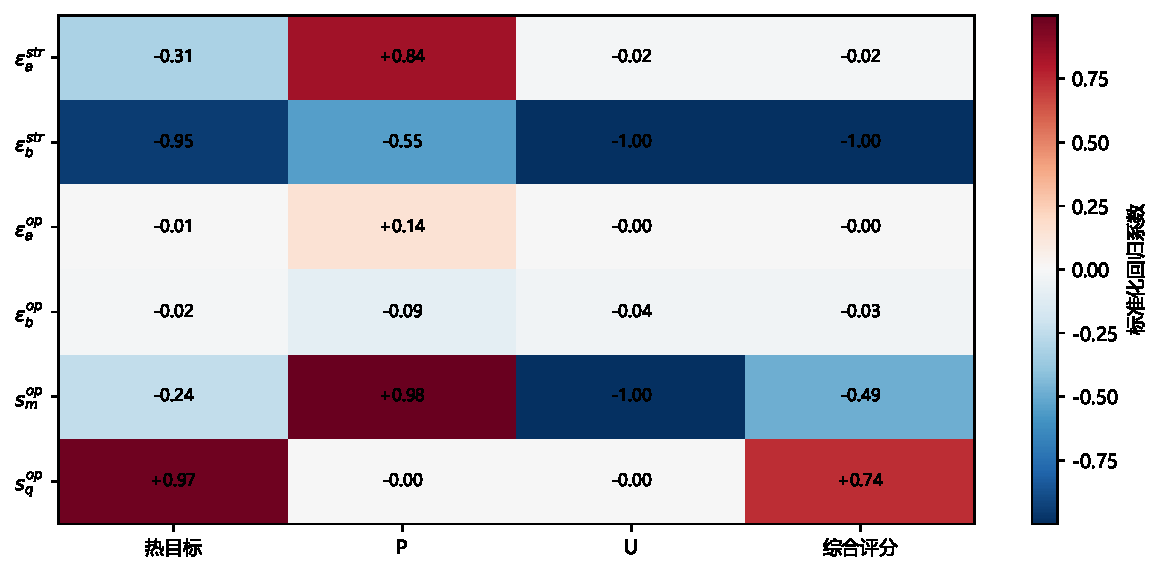
\includegraphics[width=.86\linewidth]{../../05_figures/q5/fig_q5_04_signed_sensitivity.pdf}\caption{带符号SRC；第一列在加工分析中为$R$、工况分析中为$\Theta_R$}\end{figure}
\begin{table}[H]\centering\scriptsize\caption{SRC线性近似的$R^2$}\begin{tabular}{lrrrr}\toprule 模型&热目标&P&U&综合评分\\\midrule
加工误差SRC & 0.998 & 1.000 & 0.992 & 0.992 \\
S2-A工况SRC & 1.000 & 1.000 & 1.000 & 0.787 \\\\\bottomrule\end{tabular}\end{table}
S2-A下三个单项性能的$R^2$接近1，而综合评分$R^2=.787$，说明增强切比雪夫评分的最大值算子引入分段非线性；SRC仅用于识别方向和主要影响因素，不解释为严格方差贡献率。
\subsection*{B类：工况机理情景，不替代A类结论}
工况修正定义为
\[P^{op}=\widehat P(x^r)[\alpha_Ps_m+(1-\alpha_P)s_m^2],\quad
R^{op}=\widehat R(x^r)[\theta_R+(1-\theta_R)s_m^{-m_R}],\quad \Theta_R=s_qR^{op},\]
\[U_A^{op}=\widehat U(x^r)s_m^{-m_U},\qquad U_B^{op}=\widehat U(x^r)s_qs_m^{-m_U}.\]
\begin{table}[H]\centering\scriptsize\caption{机理参数情景}\begin{tabular}{lrrrrl}\toprule 情景&$\alpha_P$&$\theta_R$&$m_R$&$m_U$&解释\\\midrule
S1&.80&.75&.25&.25&弱流量敏感\\S2&.50&.50&.50&.50&中等混合机制\\S3&.20&.25&.80&.80&强流量敏感\\\bottomrule\end{tabular}\end{table}
优化阶段对所有候选共用种子20260721生成的固定$L=3000$点LHS情景，以降低候选间Monte Carlo噪声；确定候选后，重新生成$L=12000$点LHS集作后验CVaR评价，未声称已完成24,000点收敛验证。六类结果均同时包含中等加工公差$\varepsilon_a,\varepsilon_b\sim U[-.025,.025]$与独立均匀$s_m,s_q\sim U[.95,1.05]$。评分为$C_{op}$，以$(\Theta_R,P^{op},U^{op})$按问题3固定尺度组成。
\begin{table}[H]\centering\scriptsize\caption{中等加工公差与±5\%运行波动共同作用下的机理情景结果}\begin{tabular}{llrrrrrr}\toprule 情景&U模型&a&b&N&最优CVaR&结构鲁棒CVaR&相对增幅\\\midrule
S1 & A & 0.2257 & 3.4109 & 10 & 0.96659 & 1.25857 & 30.2\% \\
S1 & B & 0.2411 & 3.0756 & 4 & 1.15690 & 1.29052 & 11.5\% \\
S2 & A & 0.2209 & 3.4841 & 10 & 1.15675 & 1.34324 & 16.1\% \\
S2 & B & 0.2408 & 3.1110 & 4 & 1.25177 & 1.42431 & 13.8\% \\
S3 & A & 0.2223 & 3.4647 & 10 & 1.42150 & 1.58066 & 11.2\% \\
S3 & B & 0.2414 & 3.0768 & 4 & 1.47820 & 1.62595 & 10.0\% \\\\\bottomrule\end{tabular}\end{table}
U模型A的低风险解集中于$N=10$，模型B集中于$N=4$，且$a\approx.22-.24,b\approx3.08-3.48$；排数对$U$的尺度定义敏感。故B类结果不能唯一确定工况专用结构。
结构鲁棒方案在六类工况下的CVaR均高于情景专属最优，说明加工鲁棒并不等同于工况鲁棒，机理形式会实质改变排数选择。在物性常数与线性传热近似下，入口温度主要平移绝对芯片温度基线；因缺少无量纲指标反归一化关系而不进入综合评分。外侧自然对流同样缺少变工况样本，保持名义值。
\begin{table}[H]\centering\scriptsize\caption{问题4--5的最终工程推荐}\begin{tabular}{p{2.3cm}p{3.0cm}p{2.5cm}p{4.2cm}}\toprule 使用条件&推荐方案&结果性质&主要结论\\\midrule
名义等权&$(.224932,4.5,6)$&域内代理优化&名义综合最优\\
权重不确定&$(.224932,4.5,6)$&偏好鲁棒&最大偏好遗憾最小\\
中等加工公差&$(.224006,4.4625,6)$&A类数据支持&避开$b=4.5$边界\\
工况模型A&$N=10$附近&B类机理情景&偏重降低热风险\\
工况模型B&$N=4$附近&B类机理情景&受热负荷缩放定义影响\\
最终工程推荐&$(.224006,4.4625,6)$&保守推荐&有数据支撑且具公差安全裕度\\\bottomrule\end{tabular}\end{table}
因此，在附件现有数据下正式采用加工鲁棒方案；待获得不同流量、热负荷下的CFD或实验数据后，再判定采用$N=4$或$N=10$的工况专用方案。\end{document}
